\documentclass[aspectratio=169]{beamer}
\usetheme{default}
\useinnertheme{circles}
\setbeamertemplate{navigation symbols}{}

\usepackage[utf8]{inputenc}
\usepackage{graphicx}

\usepackage[style=authoryear, doi=false]{biblatex}  
\addbibresource{~/Zotero/Bibliothek.bib}
\renewcommand*{\bibfont}{\tiny}

\author{Malte Grönemann}
\title{Respondent- and Interview-level predictors of Item Nonresponse in the ESS 9}
\date{20 May 2021}

\begin{document}

\begin{frame}
\maketitle
\end{frame}


\begin{frame}{Introduction}
 Missing Data are Bad
 \begin{itemize}
  \item decreases effective sample size
  \item nonresponse bias
  \item indicator of overall data quality (satisficing) \footcite{krosnickResponseStrategiesCoping1991}
 \end{itemize}
 
 \bigskip
 
 A Typology of Missingness \footcite{deleeuwPreventionTreatmentItem2003}
 \begin{itemize}
  \item missing completely at random
  \item missing at random
  \item not missing at random
  \item missing by design
 \end{itemize}
\end{frame}


\begin{frame}{Item Nonresponse}
Item nonresponse: non-substantive answer or refusal by the respondent

\bigskip

 Question-Answer-Process\footcite{deleeuwPreventionTreatmentItem2003}: understanding $\rightarrow$ recalling information $\rightarrow$  eventually judging $\rightarrow$  eventually editing $\rightarrow$  eventually formating $\rightarrow$  communicating
 
 \bigskip
 
 Two types of item nonresponse
 \begin{itemize}
  \item Don't know
  \begin{itemize}
  \item not \textit{able} to answer: mental effort is too high
   \item strategy of satisficing
   \item likely to be MAR
  \end{itemize}
\item Refusal
\begin{itemize}
 \item not \textit{wanting} to answer: privacy and sensitivity
 \item likely to be NMAR
\end{itemize}
\item But: mechanisms not perfectly separate \footcite{shoemakerItemNonresponseDistinguishing2002}
\end{itemize}
\end{frame}


\begin{frame}{Predictors of Item Nonresponse I}
 Country
 \begin{itemize}
  \item considerable country differences
  \item no good explanations to date \footcite{meitingerPowerCultureItem2020}
  \item some composition effects \footcite{kochItemNonresponseEuropean2009}
 \end{itemize}

  Survey
 \begin{itemize}
  \item compositional differences between modes \footcite{messerDeterminantsItemNonresponse2012}
  \item design possibilities and likelihood of unintended skipping
 \end{itemize}
 \end{frame}
 
 
 \begin{frame}{Predictors of Item Nonresponse II}
  Interviewer
 \begin{itemize}
  \item considerable interviewer effects
  \item barely any explanations \footcite{pickeryImpactRespondentInterviewer1998}
  \item poor interviewer behaviour?: skipping questions or shortening questionnaire
 \end{itemize}

 Respondent
 \begin{itemize}
  \item ability: age, health, education
  \item women have higher nonresponse
  \item ethnic minorities, poor language skills, low literacy
  
  $\rightarrow$ reflection of broader patterns of inequality \footcite{meitingerPowerCultureItem2020}
  \item motivation: political interest, feeling of powerlessness
 \end{itemize}
\end{frame}


 \begin{frame}{Predictors of Item Nonresponse III}
 Interview
 \begin{itemize}
  \item sometimes gender matching \footcite{vercruyssenEffectSociodemographicMis2017}
  \item similar age vs older interviewer
  \item other people present during the interview \footcite{kupekDeterminantsItemNonresponse1998}
  \item perceived cooperation of respondent \footcite{tuSocialDistanceRespondent2007}
 \end{itemize}
 
 Questionnaire
 \begin{itemize}
  \item explicitly offering DK
  \item complexity
 \end{itemize}

 Question
 \begin{itemize}
  \item sensitivity: e.g. income and sexual behaviour
 \end{itemize}

\end{frame}


\begin{frame}{Aim}
\begin{itemize}
 \item item nonresponse is still not well understood
 \item most established predictors are respondent characteristics $\rightarrow$ not changeable
 \item the aim is of course to ensure and improve data quality in the future
 \item directing attention to controlable predictors
 \item fundamental problem: data availability
 \item $\rightarrow$ explore reasonable available predictors especially on the interview level
\end{itemize}

\end{frame}


\begin{frame}{Data and Methods}
 \begin{itemize}
 \item ESS Round 9, all countries
  \item number of refusals and DK $\rightarrow$ overdispersed count data
  \item complete questionnaire excluding questions affected by routing to ensure comparability
  \item nested structure: interviews by interviewers within countries
  \item $\rightarrow$ negative binomial regression with interviewer fixed effects, standard errors clustered by interviewer
 \end{itemize}

\end{frame}


\begin{frame}{Preliminary Results}
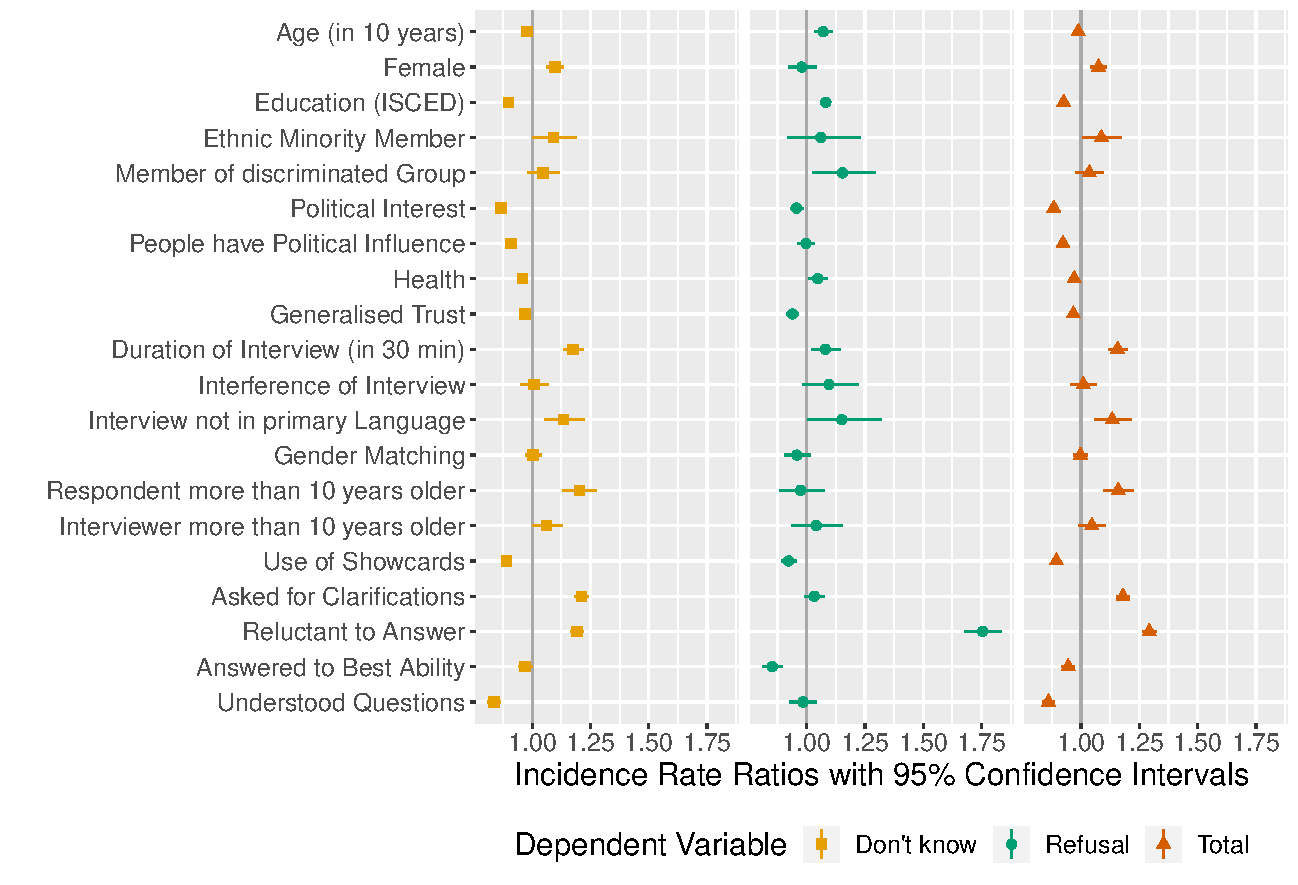
\includegraphics[scale=.35]{results.pdf}
\end{frame}


\begin{frame}{Issues}
 \begin{itemize}
  \item missing data of included variables are directly linked to value of DV $\rightarrow$ imputation?
  \item model comparisons?
  \item descriptives? (word limit...)
 \end{itemize}

\end{frame}


\begin{frame}{References}
\printbibliography
\end{frame}
\end{document}
